\documentclass{article}

\usepackage{hyperref}
\hypersetup{
	colorlinks=true,
	linkcolor=blue,
	urlcolor=cyan,}

%%%%%%%%%%%%%%%%%%%%%%%%%%%%%%%%%%%%%%%%%
% Lachaise Assignment
% Structure Specification File
% Version 1.0 (26/6/2018)
%
% This template originates from:
% http://www.LaTeXTemplates.com
%
% Authors:
% Marion Lachaise & François Févotte
% Vel (vel@LaTeXTemplates.com)
%
% License:
% CC BY-NC-SA 3.0 (http://creativecommons.org/licenses/by-nc-sa/3.0/)
% 
%%%%%%%%%%%%%%%%%%%%%%%%%%%%%%%%%%%%%%%%%

%----------------------------------------------------------------------------------------
%	PACKAGES AND OTHER DOCUMENT CONFIGURATIONS
%----------------------------------------------------------------------------------------

\usepackage{amsmath,amsfonts,stmaryrd,amssymb} % Math packages

\usepackage{enumerate} % Custom item numbers for enumerations

\usepackage[ruled]{algorithm2e} % Algorithms

\usepackage[framemethod=tikz]{mdframed} % Allows defining custom boxed/framed environments

\usepackage{listings} % File listings, with syntax highlighting
\lstset{
	basicstyle=\ttfamily, % Typeset listings in monospace font
}

%----------------------------------------------------------------------------------------
%	DOCUMENT MARGINS
%----------------------------------------------------------------------------------------

\usepackage{geometry} % Required for adjusting page dimensions and margins

\geometry{
	paper=a4paper, % Paper size, change to letterpaper for US letter size
	top=2.5cm, % Top margin
	bottom=3cm, % Bottom margin
	left=2.5cm, % Left margin
	right=2.5cm, % Right margin
	headheight=14pt, % Header height
	footskip=1.5cm, % Space from the bottom margin to the baseline of the footer
	headsep=1.2cm, % Space from the top margin to the baseline of the header
	%showframe, % Uncomment to show how the type block is set on the page
}

%----------------------------------------------------------------------------------------
%	FONTS
%----------------------------------------------------------------------------------------

\usepackage[utf8]{inputenc} % Required for inputting international characters
\usepackage[T1]{fontenc} % Output font encoding for international characters

\usepackage{XCharter} % Use the XCharter fonts

%----------------------------------------------------------------------------------------
%	COMMAND LINE ENVIRONMENT
%----------------------------------------------------------------------------------------

% Usage:
% \begin{commandline}
%	\begin{verbatim}
%		$ ls
%		
%		Applications	Desktop	...
%	\end{verbatim}
% \end{commandline}

\mdfdefinestyle{commandline}{
	leftmargin=10pt,
	rightmargin=10pt,
	innerleftmargin=15pt,
	middlelinecolor=black!50!white,
	middlelinewidth=2pt,
	frametitlerule=false,
	backgroundcolor=black!5!white,
	frametitle={Command Line},
	frametitlefont={\normalfont\sffamily\color{white}\hspace{-1em}},
	frametitlebackgroundcolor=black!50!white,
	nobreak,
}

% Define a custom environment for command-line snapshots
\newenvironment{commandline}{
	\medskip
	\begin{mdframed}[style=commandline]
}{
	\end{mdframed}
	\medskip
}

%----------------------------------------------------------------------------------------
%	FILE CONTENTS ENVIRONMENT
%----------------------------------------------------------------------------------------

% Usage:
% \begin{file}[optional filename, defaults to "File"]
%	File contents, for example, with a listings environment
% \end{file}

\mdfdefinestyle{file}{
	innertopmargin=1.6\baselineskip,
	innerbottommargin=0.8\baselineskip,
	topline=false, bottomline=false,
	leftline=false, rightline=false,
	leftmargin=2cm,
	rightmargin=2cm,
	singleextra={%
		\draw[fill=black!10!white](P)++(0,-1.2em)rectangle(P-|O);
		\node[anchor=north west]
		at(P-|O){\ttfamily\mdfilename};
		%
		\def\l{3em}
		\draw(O-|P)++(-\l,0)--++(\l,\l)--(P)--(P-|O)--(O)--cycle;
		\draw(O-|P)++(-\l,0)--++(0,\l)--++(\l,0);
	},
	nobreak,
}

% Define a custom environment for file contents
\newenvironment{file}[1][File]{ % Set the default filename to "File"
	\medskip
	\newcommand{\mdfilename}{#1}
	\begin{mdframed}[style=file]
}{
	\end{mdframed}
	\medskip
}

%----------------------------------------------------------------------------------------
%	NUMBERED QUESTIONS ENVIRONMENT
%----------------------------------------------------------------------------------------

% Usage:
% \begin{question}[optional title]
%	Question contents
% \end{question}

\mdfdefinestyle{question}{
	innertopmargin=1.2\baselineskip,
	innerbottommargin=0.8\baselineskip,
	roundcorner=5pt,
	nobreak,
	singleextra={%
		\draw(P-|O)node[xshift=1em,anchor=west,fill=white,draw,rounded corners=5pt]{%
		Question \theQuestion\questionTitle};
	},
}

\newcounter{Question} % Stores the current question number that gets iterated with each new question

% Define a custom environment for numbered questions
\newenvironment{question}[1][\unskip]{
	\bigskip
	\stepcounter{Question}
	\newcommand{\questionTitle}{~#1}
	\begin{mdframed}[style=question]
}{
	\end{mdframed}
	\medskip
}

%----------------------------------------------------------------------------------------
%	WARNING TEXT ENVIRONMENT
%----------------------------------------------------------------------------------------

% Usage:
% \begin{warn}[optional title, defaults to "Warning:"]
%	Contents
% \end{warn}

\mdfdefinestyle{warning}{
	topline=false, bottomline=false,
	leftline=false, rightline=false,
	nobreak,
	singleextra={%
		\draw(P-|O)++(-0.5em,0)node(tmp1){};
		\draw(P-|O)++(0.5em,0)node(tmp2){};
		\fill[black,rotate around={45:(P-|O)}](tmp1)rectangle(tmp2);
		\node at(P-|O){\color{white}\scriptsize\bf !};
		\draw[very thick](P-|O)++(0,-1em)--(O);%--(O-|P);
	}
}

% Define a custom environment for warning text
\newenvironment{warn}[1][Warning:]{ % Set the default warning to "Warning:"
	\medskip
	\begin{mdframed}[style=warning]
		\noindent{\textbf{#1}}
}{
	\end{mdframed}
}

%----------------------------------------------------------------------------------------
%	INFORMATION ENVIRONMENT
%----------------------------------------------------------------------------------------

% Usage:
% \begin{info}[optional title, defaults to "Info:"]
% 	contents
% 	\end{info}

\mdfdefinestyle{info}{%
	topline=false, bottomline=false,
	leftline=false, rightline=false,
	nobreak,
	singleextra={%
		\fill[black](P-|O)circle[radius=0.4em];
		\node at(P-|O){\color{white}\scriptsize\bf i};
		\draw[very thick](P-|O)++(0,-0.8em)--(O);%--(O-|P);
	}
}

% Define a custom environment for information
\newenvironment{info}[1][Info:]{ % Set the default title to "Info:"
	\medskip
	\begin{mdframed}[style=info]
		\noindent{\textbf{#1}}
}{
	\end{mdframed}
}
 % Include the file specifying the document structure and custom commands

%----------------------------------------------------------------------------------------
%	ASSIGNMENT INFORMATION
%----------------------------------------------------------------------------------------

\title{Project 2: EMG Reflex Assignment (EMG)}
\author{BIOE 385 Bioinstrumentation Laboratory} 
\date{}
%----------------------------------------------------------------------------------------

\begin{document}
\large
\maketitle
\section*{Introduction}
You are a research engineer working at a major hospital in the Texas Medical Center. Your boss is interested in studying the reflex time associated with muscle response in patients with various neurological conditions. Your job is to create the biomedical instrumentation and documentation that is required to conduct the study.\\

\begin{figure}[h]
    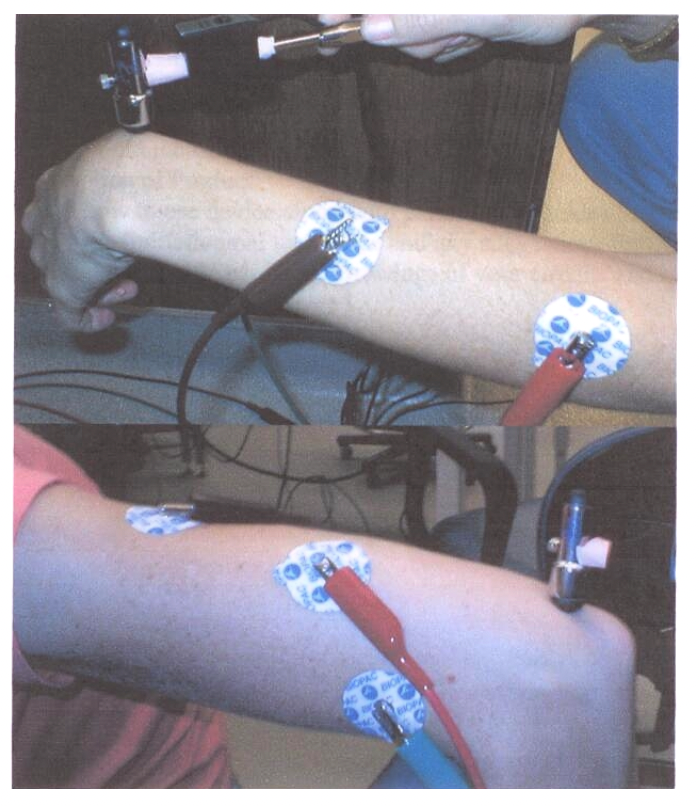
\includegraphics[width=0.4\textwidth]{emg_fig_1.png}
    \centering
\label{fig_1}
\end{figure}

\section*{Assignment}

The following features are necessary in your device:
\begin{itemize}
	\item The EMG signal must be collected with a circuit you design.
	\item You will have an instrumented reflex hammer for which you must also design appropriate circuitry.
	\item Each of these signals should be amplified and filtered appropriately and then collected simultaneously.
	\item You will display the data using LabView, and the user must be able to determine EASILY (if not in an automated manner) the time between the hammer strike and the muscle response.
\end{itemize}

\section*{Report Draft}
Each group will turn in a report draft for their EMG-Hammer device (\href{https://github.com/jlongc12/BIOE_385/blob/main/general_course_materials/syllabus.pdf}{see schedule in syllabus}). This draft will be evaluated by your peers and the instructor. The grade obtained in this assignment, as well as the quality of your evaluation of another group’s device, will contribute 20 points towards your grade.\\

The report draft will consist of 2 parts:
\begin{enumerate}
	\item \textbf{User Manual}
	
	You must write a User Manual that enables a health care professional such as a paramedic or nurse to setup and run the device (\textit{only hardware}) without any previous training.\\
	
	Minimum requirements:
	\begin{itemize}
		\item Detailed table of contents for all sections included in the draft
		\item Summary and description of your device (\textit{only hardware})
		\item Clear instructions explaining how to setup and use the device along with pictures and guides that are easy to follow (\textit{only hardware})
	\end{itemize}
	
	\item \textbf{Technical Specifications}
	
	The second part of the report should include technical specifications that allow other engineering teams to understand how your device is designed, modify it and make further improvements when necessary.\\
	
	Minimum requirements:
	\begin{itemize}
		\item Appendices that include drawings of your circuits and explanations of technical aspects of the device.
		\item Challenges associated with the interaction between living and non-living systems.
	\end{itemize}
\end{enumerate}

Longer is NOT better for the purposes of this assignment. A clear, concise, well-written report is preferred. Be sure to review the detailed grading rubric for your report draft in the course website.

\pagebreak

\section*{Final Report}
During the last week, each group will turn in a final EMG-Hammer Report for their device. You will also have the opportunity to demonstrate your device as part of the end of project test.\\

The final report will consist of 2 parts:
\begin{enumerate}
	\item \textbf{User Manual}
	
	You must write a User Manual that enables a health care professional such as a paramedic or nurse to setup and run the device (\textit{hardware and LabView program}) without any previous training.\\
	
	Minimum requirements:
	\begin{itemize}
		\item Detailed table of contents
		\item Summary and description of your device 
		\item Clear instructions explaining how to setup and use the device along with pictures and guides that are easy to follow
	\end{itemize}
	
	\item \textbf{Technical Specifications}
	
	The second part of the report should include technical specifications that allow other engineering teams to understand how your device is designed, modify it and make further improvements when necessary.\\
	
	Minimum requirements:
	\begin{itemize}
		\item Clear descriptions of the limitations of the device and any suggestions for improvements.
		\item Appendices that include the LabView Code, drawings of your circuits, and explanations of technical aspects of the device.
		\item Challenges associated with the interaction between living and non-living systems.
	\end{itemize}
\end{enumerate}

Longer is NOT better for the purposes of this assignment. A clear, concise, well-written report is preferred. Be sure to review the detailed grading rubric for your final report in the course website.

\pagebreak
\section*{Learning Objectives}
\subsection*{Lab 1}
Students should be able to:
\begin{itemize}
	\item Use NI ELVIS Bode Analyzer to obtain a plot that describes a filter’s response
	\item Explain the time constant and how voltage changes in an RC circuit as a function of time.
	\item Design and build passive filters (low-pass, high-pass, band-pass and band-stop) given a desired cut-off frequency
	\item Design and build active filters (low-pass, high-pass, band-pass and band-stop) given a desired cut-off frequency
	\item Explain the differences between active and passive filters
	\item Explain the differences between lower-order and higher-order filters
	\item Explain the differences between low-pass, high-pass, band-pass and band-stop filters
	\item Calculate the cutoff-frequency and time constant of a given filter 
\end{itemize}

\subsection*{Lab 2}
Students should be able to:
\begin{itemize}
	\item Design and build a circuit to measure the output from a reflex hammer
	\item Calculate the gain and build circuits to amplify voltage using inverting, non-inverting and differential amplifiers
	\item Solder electrical components 
\end{itemize}

\subsection*{Lab 3}
Students should be able to:
\begin{itemize}
	\item Determine the amplitude and frequency range of an EMG signal
	\item Explain how the electrical isolation circuit built in class works to protect the patient from the risk of exposure to high voltages or currents in the event of component failure
	\item Design a circuit to amplify and filter an EMG signal
	\item Justify the selection of components used to amplify the EMG signal (ie. 2-stage amplification, gain, instrumentation amplifiers, etc)
	\item Use OP07 and AD620 instrumentation amplifiers to design circuits.  
\end{itemize}

\subsection*{Lab 4}
Students should be able to:
\begin{itemize}
	\item Modify properties of the DAQ to acquire the desired data
	\item Create digital filters using LabView
	\item Modify properties of waveform graphs and charts to correctly display the desired data (display correct labels, units, scaling, etc)
	\item Measure the time associated with a specific event using time stamps, counting iterations OR using other methods that allow a millisecond resolution
	\item Use a variety of controls and indicators to create an easy to use VI
\end{itemize}

\subsection*{Lab 5}
Students should be able to:
\begin{itemize}
	\item Set default values for indicators and control the range (maximum and/or minimum value) that the user can manipulate
	\item Display data from different channels in the same graph or chart
	\item Merge and split signals
	\item Store results in a table (front panel) and save them into a file
	\item Use Inputs from the Express functions in LabView to acquire and simulate signals
	\item Use Structures, Arrays, Numeric, Boolean, Comparison, File I/O, Timing and Strings from the Programming functions in LabView to create user friendly VIs
	\item Justify the selection of components used in the circuits designed in lab
	\item Explain the LabView VI built to calculate reflex time
	\item Identify and describe the main limitations of your device
\end{itemize}
\end{document}
